\documentclass[../../relatorio.tex]{subfiles}
\begin{document}
Foram construídas várias classes de implementação, nomeadamente: 
\textit{Precos}, \textit{CustoTotalReparacao},
\textit{ReparacoesPorMes} e \textit{GestAgenda}.

\subsubsection*{Precos} \label{class:precos}
Constituída unicamente por variáveis e métodos estáticos, permite
armazenar o custo da hora do técnico.
O objetivo desta classe é que ao criar um novo orçamento, seja copiado para o orçamento
o valor horário do técnico e garantir que, mesmo havendo flutuações do custo
da mão de obra, estes não irão afetar o valor do orçamento.

Optou-se por colocar desta forma para que haja maior facilidade de acesso ao valor,
por qualquer classe.

\begin{figure} [!ht]
    \centering
    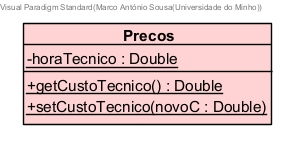
\includegraphics[scale=0.5]{precos.jpg}
    \caption{Precos}\label{img:precos}
\end{figure}

\subsubsection*{CustoTotalReparacao} \label{class:custo_total_reparacao}
Classe auxiliar que permite calcular o preço total de uma reparação,
assim como o desvio de tempo em relação ao estimado.
A sua utilização consiste em, depois de ser instanciada, adicionar um novo passo
(tempo, tempoEstimado e custoMaterial).

Sempre que recebe um novo passo, os parâmetros recebidos são adicionados
aos acumuladores de instância.

No fundo, esta classe serve como um acumulador que centraliza as operações e
devolve várias informações sobre a reparação.

\begin{figure} [!ht]
    \centering
    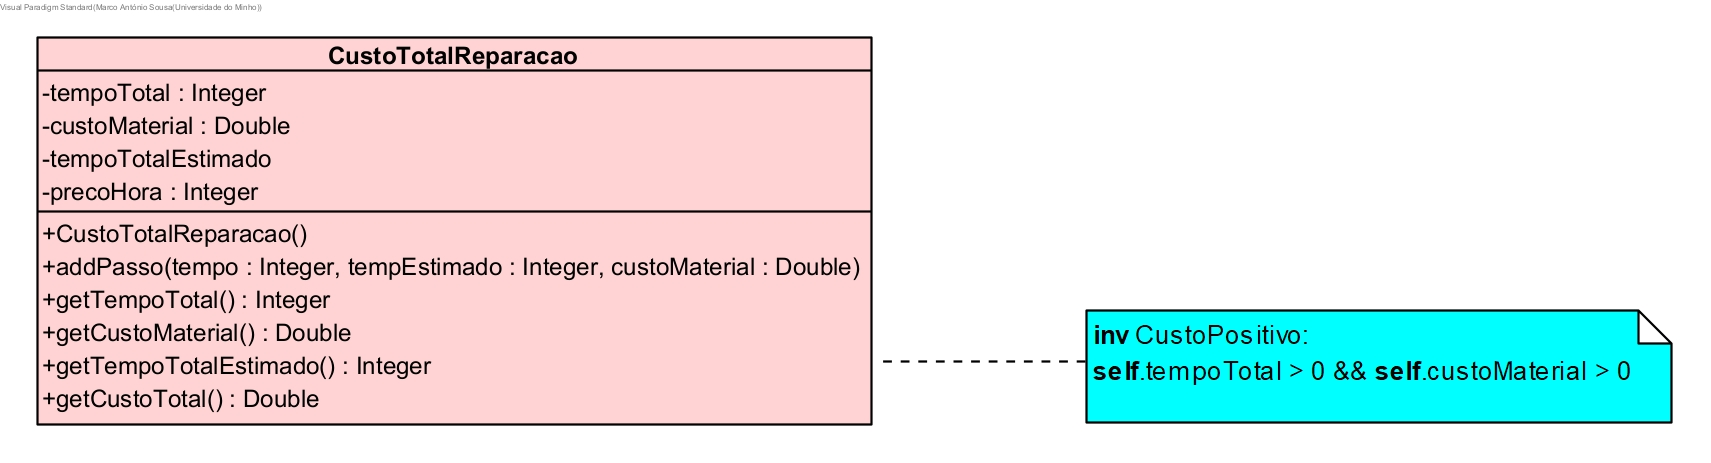
\includegraphics[width=\linewidth]{custoTotalReparacao.jpg}
    \caption{Custo Total Reparacao}\label{img:custo_total_reparacao}
\end{figure}

\subsubsection*{ReparacoesPorMes} \label{class:reparacoes_por_mes}
Tal como o anterior, esta classe também tem como finalidade servidor de acumulador.
No entanto, trata-se de um acumulador um pouco mais complexo, no sentido
em que sempre que é adicionado uma nova reparação, calcula a sua duração
e atualiza duas médias: duração média das reparações e média do desvio
da duração das reparação em relação ao esperado.
Para tal, é utilizado a média ponderada entre o acumulador e novo valor a acrescentar,
mantendo uma variável auxiliar que é o total.

\begin{figure} [!ht]
    \centering
    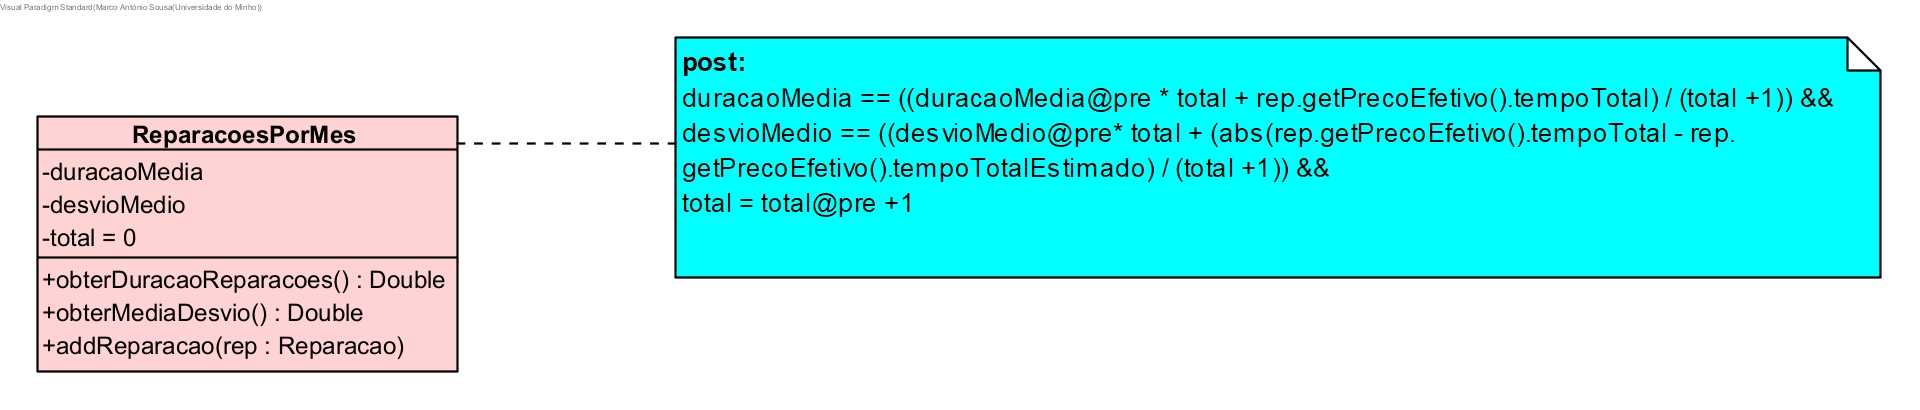
\includegraphics[width=\linewidth]{reparacoesPorMes.jpg}
    \caption{Reparacoes Por Mes}\label{img:reparacoes_por_mes}
\end{figure}

\subsubsection*{GestAgenda} \label{class:gest_agenda}

\end{document}